% Created by tikzDevice version 0.10.1 on 2017-11-26 21:00:39
% !TEX encoding = UTF-8 Unicode
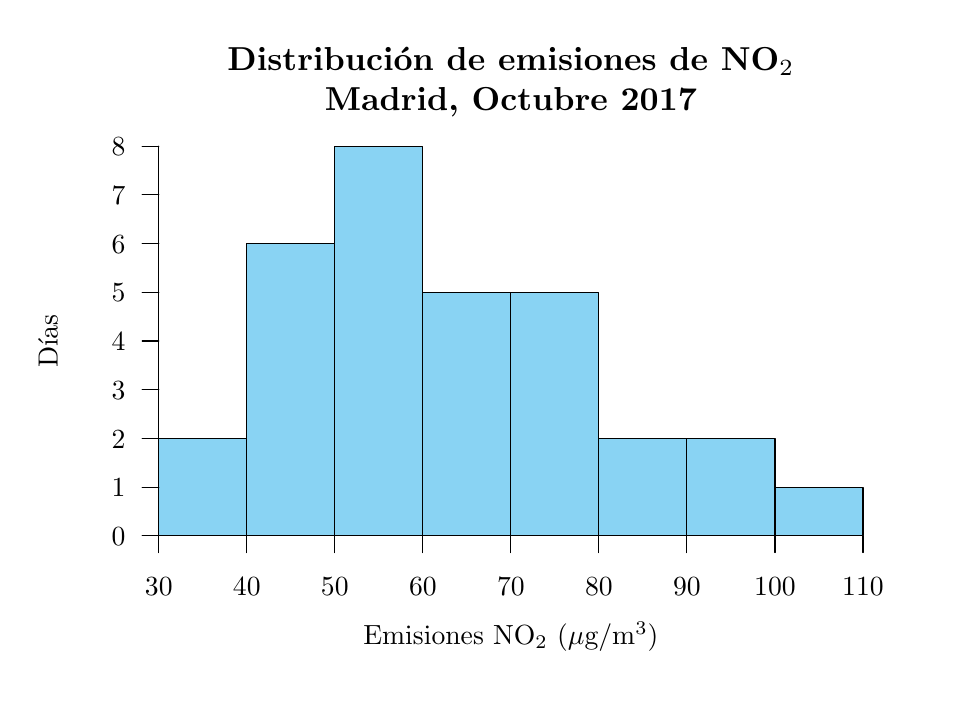
\begin{tikzpicture}[x=1pt,y=1pt]
\definecolor{fillColor}{RGB}{255,255,255}
\path[use as bounding box,fill=fillColor,fill opacity=0.00] (0,0) rectangle (325.21,238.49);
\begin{scope}
\path[clip] (  0.00,  0.00) rectangle (325.21,238.49);
\definecolor{drawColor}{RGB}{0,0,0}

\node[text=drawColor,anchor=base,inner sep=0pt, outer sep=0pt, scale=  1.20] at (174.61,222.95) {\bfseries Distribución de emisiones de NO$_2$};

\node[text=drawColor,anchor=base,inner sep=0pt, outer sep=0pt, scale=  1.20] at (174.61,208.55) {\bfseries  Madrid, Octubre 2017};

\node[text=drawColor,anchor=base,inner sep=0pt, outer sep=0pt, scale=  1.00] at (174.61, 15.60) {Emisiones NO$_2$ ($\mu$g/m$^3$)};

\node[text=drawColor,rotate= 90.00,anchor=base,inner sep=0pt, outer sep=0pt, scale=  1.00] at ( 10.80,125.25) {Días};
\end{scope}
\begin{scope}
\path[clip] ( 37.20, 49.20) rectangle (312.01,201.29);
\definecolor{drawColor}{RGB}{0,0,0}
\definecolor{fillColor}{RGB}{137,211,243}

\path[draw=drawColor,line width= 0.4pt,line join=round,line cap=round,fill=fillColor] ( 47.38, 54.83) rectangle ( 79.19, 90.04);

\path[draw=drawColor,line width= 0.4pt,line join=round,line cap=round,fill=fillColor] ( 79.19, 54.83) rectangle (110.99,160.45);

\path[draw=drawColor,line width= 0.4pt,line join=round,line cap=round,fill=fillColor] (110.99, 54.83) rectangle (142.80,195.66);

\path[draw=drawColor,line width= 0.4pt,line join=round,line cap=round,fill=fillColor] (142.80, 54.83) rectangle (174.61,142.85);

\path[draw=drawColor,line width= 0.4pt,line join=round,line cap=round,fill=fillColor] (174.61, 54.83) rectangle (206.41,142.85);

\path[draw=drawColor,line width= 0.4pt,line join=round,line cap=round,fill=fillColor] (206.41, 54.83) rectangle (238.22, 90.04);

\path[draw=drawColor,line width= 0.4pt,line join=round,line cap=round,fill=fillColor] (238.22, 54.83) rectangle (270.03, 90.04);

\path[draw=drawColor,line width= 0.4pt,line join=round,line cap=round,fill=fillColor] (270.03, 54.83) rectangle (301.84, 72.44);
\end{scope}
\begin{scope}
\path[clip] (  0.00,  0.00) rectangle (325.21,238.49);
\definecolor{drawColor}{RGB}{0,0,0}

\path[draw=drawColor,line width= 0.4pt,line join=round,line cap=round] ( 47.38, 54.83) -- (301.84, 54.83);

\path[draw=drawColor,line width= 0.4pt,line join=round,line cap=round] ( 47.38, 54.83) -- ( 47.38, 48.83);

\path[draw=drawColor,line width= 0.4pt,line join=round,line cap=round] ( 79.19, 54.83) -- ( 79.19, 48.83);

\path[draw=drawColor,line width= 0.4pt,line join=round,line cap=round] (110.99, 54.83) -- (110.99, 48.83);

\path[draw=drawColor,line width= 0.4pt,line join=round,line cap=round] (142.80, 54.83) -- (142.80, 48.83);

\path[draw=drawColor,line width= 0.4pt,line join=round,line cap=round] (174.61, 54.83) -- (174.61, 48.83);

\path[draw=drawColor,line width= 0.4pt,line join=round,line cap=round] (206.41, 54.83) -- (206.41, 48.83);

\path[draw=drawColor,line width= 0.4pt,line join=round,line cap=round] (238.22, 54.83) -- (238.22, 48.83);

\path[draw=drawColor,line width= 0.4pt,line join=round,line cap=round] (270.03, 54.83) -- (270.03, 48.83);

\path[draw=drawColor,line width= 0.4pt,line join=round,line cap=round] (301.84, 54.83) -- (301.84, 48.83);

\node[text=drawColor,anchor=base,inner sep=0pt, outer sep=0pt, scale=  1.00] at ( 47.38, 33.23) {30};

\node[text=drawColor,anchor=base,inner sep=0pt, outer sep=0pt, scale=  1.00] at ( 79.19, 33.23) {40};

\node[text=drawColor,anchor=base,inner sep=0pt, outer sep=0pt, scale=  1.00] at (110.99, 33.23) {50};

\node[text=drawColor,anchor=base,inner sep=0pt, outer sep=0pt, scale=  1.00] at (142.80, 33.23) {60};

\node[text=drawColor,anchor=base,inner sep=0pt, outer sep=0pt, scale=  1.00] at (174.61, 33.23) {70};

\node[text=drawColor,anchor=base,inner sep=0pt, outer sep=0pt, scale=  1.00] at (206.41, 33.23) {80};

\node[text=drawColor,anchor=base,inner sep=0pt, outer sep=0pt, scale=  1.00] at (238.22, 33.23) {90};

\node[text=drawColor,anchor=base,inner sep=0pt, outer sep=0pt, scale=  1.00] at (270.03, 33.23) {100};

\node[text=drawColor,anchor=base,inner sep=0pt, outer sep=0pt, scale=  1.00] at (301.84, 33.23) {110};

\path[draw=drawColor,line width= 0.4pt,line join=round,line cap=round] ( 47.38, 54.83) -- ( 47.38,195.66);

\path[draw=drawColor,line width= 0.4pt,line join=round,line cap=round] ( 47.38, 54.83) -- ( 41.38, 54.83);

\path[draw=drawColor,line width= 0.4pt,line join=round,line cap=round] ( 47.38, 72.44) -- ( 41.38, 72.44);

\path[draw=drawColor,line width= 0.4pt,line join=round,line cap=round] ( 47.38, 90.04) -- ( 41.38, 90.04);

\path[draw=drawColor,line width= 0.4pt,line join=round,line cap=round] ( 47.38,107.64) -- ( 41.38,107.64);

\path[draw=drawColor,line width= 0.4pt,line join=round,line cap=round] ( 47.38,125.25) -- ( 41.38,125.25);

\path[draw=drawColor,line width= 0.4pt,line join=round,line cap=round] ( 47.38,142.85) -- ( 41.38,142.85);

\path[draw=drawColor,line width= 0.4pt,line join=round,line cap=round] ( 47.38,160.45) -- ( 41.38,160.45);

\path[draw=drawColor,line width= 0.4pt,line join=round,line cap=round] ( 47.38,178.05) -- ( 41.38,178.05);

\path[draw=drawColor,line width= 0.4pt,line join=round,line cap=round] ( 47.38,195.66) -- ( 41.38,195.66);

\node[text=drawColor,anchor=base east,inner sep=0pt, outer sep=0pt, scale=  1.00] at ( 35.38, 51.39) {0};

\node[text=drawColor,anchor=base east,inner sep=0pt, outer sep=0pt, scale=  1.00] at ( 35.38, 68.99) {1};

\node[text=drawColor,anchor=base east,inner sep=0pt, outer sep=0pt, scale=  1.00] at ( 35.38, 86.60) {2};

\node[text=drawColor,anchor=base east,inner sep=0pt, outer sep=0pt, scale=  1.00] at ( 35.38,104.20) {3};

\node[text=drawColor,anchor=base east,inner sep=0pt, outer sep=0pt, scale=  1.00] at ( 35.38,121.80) {4};

\node[text=drawColor,anchor=base east,inner sep=0pt, outer sep=0pt, scale=  1.00] at ( 35.38,139.41) {5};

\node[text=drawColor,anchor=base east,inner sep=0pt, outer sep=0pt, scale=  1.00] at ( 35.38,157.01) {6};

\node[text=drawColor,anchor=base east,inner sep=0pt, outer sep=0pt, scale=  1.00] at ( 35.38,174.61) {7};

\node[text=drawColor,anchor=base east,inner sep=0pt, outer sep=0pt, scale=  1.00] at ( 35.38,192.21) {8};
\end{scope}
\end{tikzpicture}
